% !TeX spellcheck = en_US
%%% Version 2.5 Generated 2018/06/15 %%%
%%% You will need to have the following packages installed: datetime, fmtcount, etoolbox, fcprefix, which are normally inlcuded in WinEdt. %%%
%%% In http://www.ctan.org/ you can find the packages and how to install them, if necessary. %%%
%%%  NB logo1.jpg is required in the path in order to correctly compile front page header %%%

\documentclass[utf8,sort&compress,numbers,square,table,hidelinks]{frontiers_suppmat} % for all articles
\usepackage{url,hyperref,lineno,microtype}
\usepackage[onehalfspacing]{setspace}
\usepackage{xcolor}
\usepackage{xspace}
\usepackage{listings}
\usepackage{multicol}
\usepackage[normalem]{ulem}
\usepackage{booktabs}

\newcommand{\todo}{\colorbox{red!30}{TODO}\xspace}
\newcommand{\review}[1]{\textcolor{red}{#1}}

\graphicspath{ {./figures/} }

% Leave a blank line between paragraphs instead of using \\

\begin{document}
\onecolumn
\firstpage{1}

\title[Supplementary Information]{{\helveticaitalic{Supplementary Information}}}

\maketitle

\vspace*{6pt}
\section{Data Sources}
\label{sec:data}

\vspace*{6pt}
\subsection{United States Statutes}

For statutes in the United States, 
we use the United States Code (USC) as our data source. 
The USC is a compilation of the general and permanent laws of the United States on the federal level, excluding state legislation.
The Office of the Law Revision Counsel of the U.S. House of Representatives (henceforth: the Office) updates the Code continuously and publishes annual versions (although the codification process can lag behind the state of the law by several years). 
When Congress passes new legislation, 
this legislation is initially published as a \emph{Slip Law} in the \emph{United States Statutes at Large}. 
If the new legislation is considered general and permanent law, the Office integrates the law into the USC.
Depending on the Titles of the Code that are modified, 
the work of the Office is approved by Congress, 
whereby the \emph{Slip Law} is repealed and replaced by the USC as the new primary source of the law. 
Even if the work of the Office is not approved by Congress, the USC is still presumed to be the correct consolidation of the law.

We base our work on the Annual Historical Archives published by the Office, 
which are available on its website.\footnote{\url{https://uscode.house.gov/download/annualhistoricalarchives/annualhistoricalarchives.htm}.}
The USC is provided in a documented (X)HTML.\footnote{\url{https://uscode.house.gov/download/resources/USLM-User-Guide.pdf}.} 
This format is flexible and offers a wide variety of styles to closely represent the printed code. 
The Code is split into single files per year and Title.
The Annual Historical Archives date back until $1994$, 
and they are published with delay. 
As of January $2021$, therefore, $2019$ is the latest available edition.

While surveying and validating the raw data, we observe and correct the following obvious errors:
\begin{itemize}
	\item double-closing \texttt{<div>}-Tags in Title~40 in $2008$, and in Title~42 in $1994$ and $1995$,
	\item inconsistent metadata in the appendix of Title~28 in $2017$,
	\item a duplicate of Title~12 in $1998$ that is included in the files for Title~11 and Title~12, 
	\item inconsistencies regarding the tags \texttt{<statute>} and the comments \texttt{<!-- \/section-head -->}, and
	\item nesting errors in Title 42 in $1999$, $2005$, $2006$ and $2007$ that caused some sections from Chapter~85 ($1999$) or 149 ($2005$--$2007$) to lie outside of their chapter.
\end{itemize}	
	
This data source is nearly identical to the source used in \cite{katz2020}, 
but the inspected time frame is updated.

\vspace*{6pt}
\subsection{United States Regulations}
\label{subsec:uscfr}

For regulations in the United States,
we use the Code of Federal Regulations (CFR) as our data source. 
The CFR is a codification of the general and permanent rules published in the Federal Register by the departments and agencies of the Federal Government, excluding regulations below the federal level and other (e.g., less permanent) regulations.
Like the USC, the CFR is updated continuously, and the codification process can lag behind the state of the law by several years.

Our work is based on the annual bulk data provided by the U.S. Government Publishing Office (GPO) in partnership with the National Archives’ Office of the Federal Register (OFR), which is available from their website.\footnote{\url{https://www.govinfo.gov/bulkdata/CFR/}.}
The data is provided in a documented XML format,\footnote{\url{https://www.govinfo.gov/bulkdata/CFR/resources/CFR-XML_User-Guide_v1.pdf};\newline \url{https://github.com/usgpo/bulk-data}.} 
whose structure is influenced by the printed version of the CFR. 
It contains one file per year and Volume of the (printed) CFR.
The data dates back until $1996$, and it is published with delay. 
Since the first two published years of the data are incomplete, we start our analysis in $1998$ (for all data sources).

Unfortunately, in the bulk downloads for some years, especially for the year $2002$, some CFR Volumes are missing although they reappear in later years, i.e., there are gaps in the data. 
We fill these gaps using the data of the closest previous year in which the Volume is available. 
This corresponds to the \emph{forward fill} strategy to complete missing data, with the modification that we only fill \emph{gaps}, 
i.e., we require that a Volume exists in an earlier snapshot and in a later snapshot (e.g., since Title~50 Volume~14 only exists in $2013$, we do not fill any gaps regarding this volume).
In other words, we inspect collections of the most recent versions of CFR Volumes at a given point in time.  
In Figures~\ref{fig:missing-cfr-volumes-1}--\ref{fig:missing-cfr-volumes-3}, we show the Volumes included in the bulk download \emph{before} filling the gaps as described above. 
The figures also illustrate the incompleteness of the data in $1996$, $1997$, and $2020$, 
and the increase in the number of Volumes for Title~40 and Title~50 is striking. 
When interpreting the figures, it is important to note that all Volumes are visualized as rectangles with the same, fixed area, although their text lengths vary widely.

\begin{figure}
	\centering
	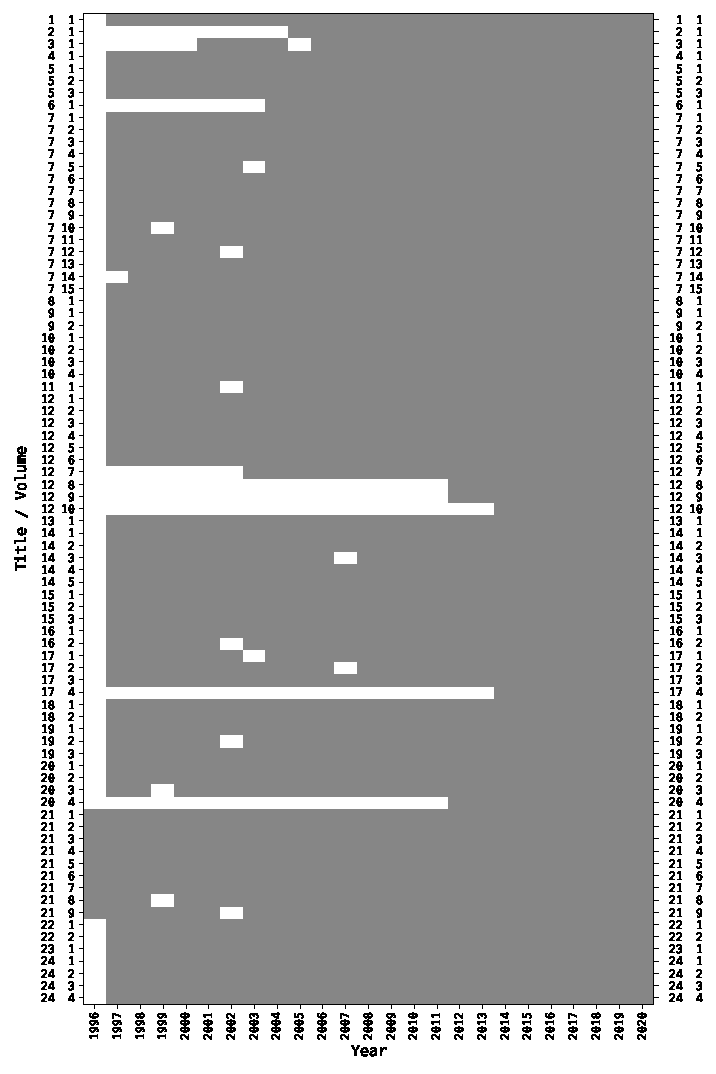
\includegraphics[height=0.9\textheight]{figure_si_cfr_inputs-0}
	\caption{Volumes of the CFR that are included in the data source. The y-axis is ordered by title and volume. (1 of 3)}\label{fig:missing-cfr-volumes-1}
\end{figure}

\begin{figure}
	\centering
	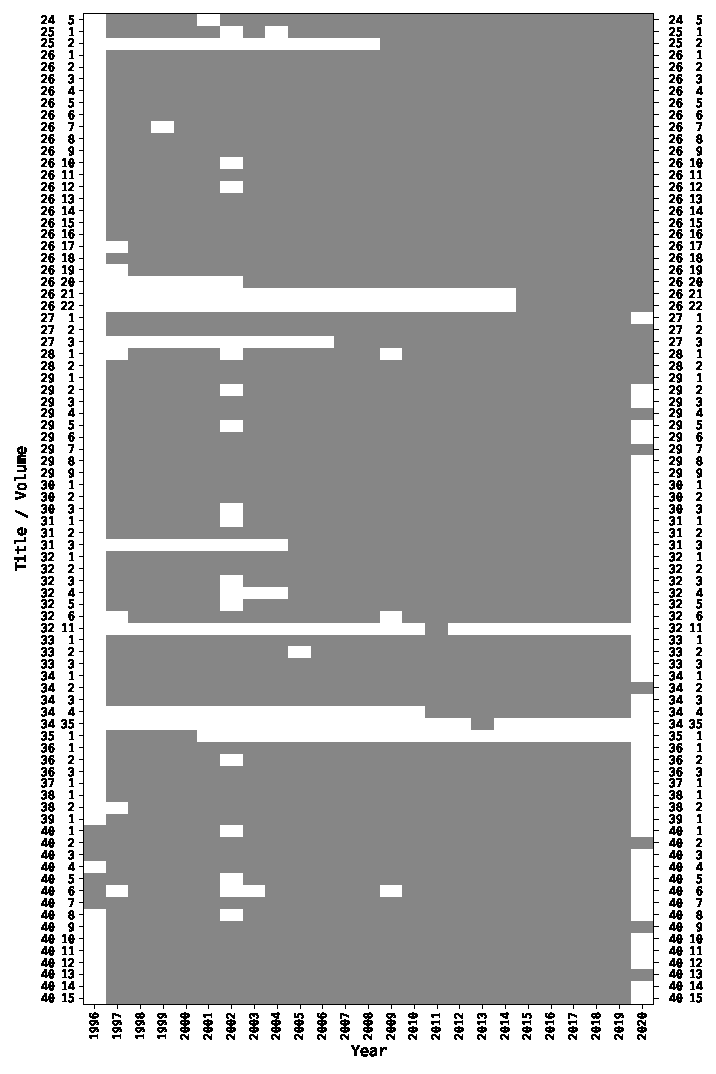
\includegraphics[height=0.9\textheight]{figure_si_cfr_inputs-1}
	\caption{Volumes of the CFR that are included in the data source. The y-axis is ordered by title and volume. (2 of 3)}\label{fig:missing-cfr-volumes-2}
\end{figure}


\begin{figure}
	\centering
	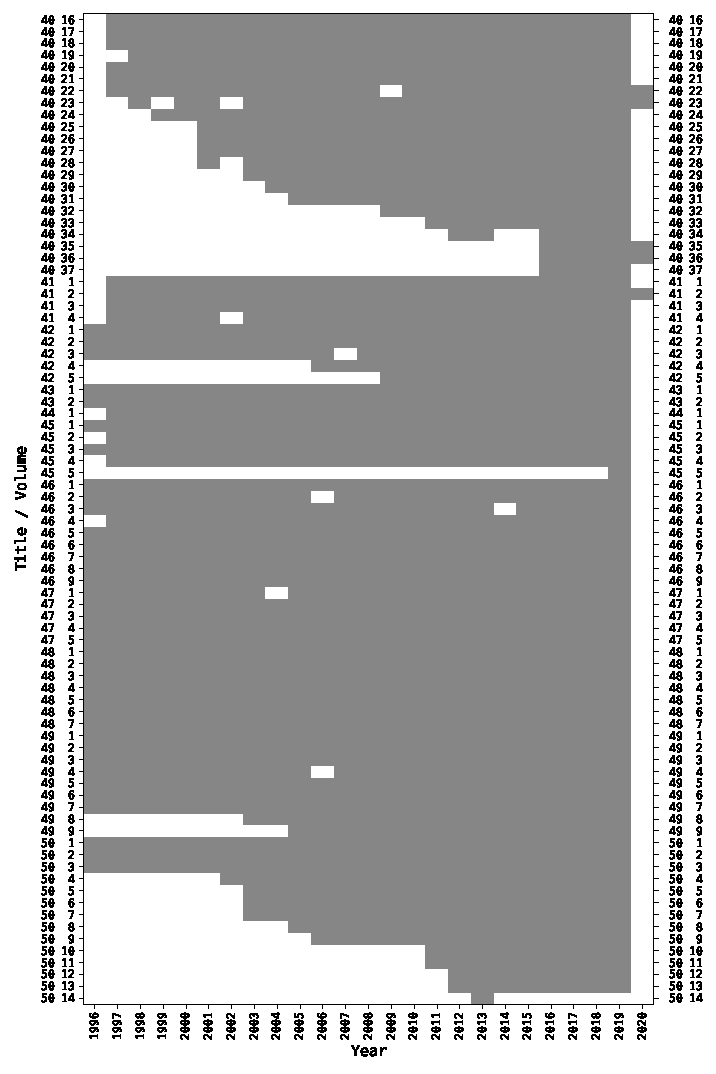
\includegraphics[height=0.9\textheight]{figure_si_cfr_inputs-2}
	\caption{Volumes of the CFR that are included in the data source. The y-axis is ordered by title and volume. (3 of 3)}\label{fig:missing-cfr-volumes-3}
\end{figure}

\vspace*{6pt}
\subsection{German Statutes and Regulations}

In Germany,
all federal statutes and regulations are published in the Federal Law Gazette as amending laws,
which often combine introductions of new statutes or regulations with amendments to and repeals of existing laws.
Individual statutes and regulations are officially classified into one of nine substantive categories with currently $73$ sub-categories that contain over $400$ subject areas in the ``Fundstellennachweis~A'' (\emph{Finding Aids A}).
The Finding Aids A are published annually by the Federal Law Gazette upon instruction by the Ministry of Justice.
However, unlike the USC, there is no official data source that provides all compiled general and permanent laws at the federal level along with their historical versions.
Here, we profit from a generous cooperation with the leading German legal data provider, \emph{juris GmbH}, 
to obtain a dataset similar to the annual versions of the USC and CFR. 
Although \emph{juris} is a private company, 
the Federal Republic of Germany is its majority shareholder, 
and all branches of government rely heavily on \emph{juris} to process legislative data. 
According to \emph{juris}, the database contains every German federal statute and regulation since spring $1990$.
The data is not as structured as the USC data or the CFR data.
Instead of maintaining annual consolidated versions,
\emph{juris} stores a new version of a statute and regulation for all changes that take effect on the same day.
The data we use comes in separate files for each law and version.
Thus, for German statutes, our data source is identical to that used in \cite{katz2020},
but the inspected time frame is updated.

We may not share the text content of the German data along with this paper.
However, a website maintained by the German Federal Ministry of Justice and Consumer Protection in collaboration with \emph{juris}
provides almost the entire federal legislation as XML files in the most recent version (i.e., without historical versions).\footnote{\url{https://www.gesetze-im-internet.de}.}
A daily archive of the XML files provided on this website (starting in June $2019$) is maintained by the QuantLaw research group.\footnote{\url{https://github.com/QuantLaw/gesetze-im-internet}.}
This dataset allows a partial reproduction of the research with a similar dataset.
We requested the full dataset from \emph{juris GmbH}, 
which required a dedicated contractual framework and non-disclosure agreement to be signed.

\clearpage

\vspace*{6pt}
\section{Samples of Legal Texts}
\label{sec:textsamples}

The following fragments illustrate the inherent structure of legal texts. 
Hierarchical inclusion relationships are indicated by indentation, 
labels of items on the documents' sequence level (\emph{seqitems}) are typeset in \textsc{small capitals}, 
references are \uline{underlined},
and text content is set in \emph{Italics}.\\

\vspace*{6pt}
\subsection{United States Statutes}

\vspace*{6pt}\noindent\hspace*{0.04\textwidth}\fbox{
	\parbox{0.9\textwidth}{%
		\textbf{United States Code (2018 Main Edition and Supplement I)}
		
		\hspace*{1em}Title 12—Banks and Banking
		
		\hspace*{2em}Chapter 53—Wall Street Reform and Consumer Protection
		
		\hspace*{3em}Subchapter I—Financial Stability
		
		\noindent\hangindent4em\hspace{4em}Part C—Additional Board of Governors Authority for Certain Nonbank Financial Companies and Bank Holding Companies
		
		\hspace*{5em}\textsc{§~5363. Acquisitions}
			
		\hspace*{6em}(a) Acquisitions of Bank; Treatment as a Bank Holding Company
		
		\noindent\hangindent7em\hspace{7em}\emph{For purposes of \uline{section 1842 of this title}, a nonbank financial company supervised by the Board of Governors shall be deemed to be, and shall be treated as, a bank holding company.}
		
		\hspace*{6em}(b) Acquisition of Nonbank Companies
		
		\hspace*{7em}(1) Prior Notice for Large Acquisitions
		
		\noindent\hangindent8em\hspace{8em}\emph{Notwithstanding \uline{section 1843(k)(6)(B) of this title}, a bank holding company with total consolidated assets equal to or greater than \$$250,000,000,000$ or a nonbank financial company supervised by the Board of Governors shall not acquire direct or indirect ownership or control of any voting shares of any company (other than an insured depository institution) that is engaged in activities described in \uline{section 1843(k) of this title} having total consolidated assets of \$$10,000,000,000$ or more, without providing written notice to the Board of Governors in advance of the transaction.}
		
		\hspace*{7em}\dots
		
		\hspace*{6em}\dots
		
		\noindent\hangindent5em\hspace*{5em}\textsc{§~5364. Prohibition against management interlocks between certain financial companies}
		
		\noindent\hangindent6em\hspace{6em}\emph{A nonbank financial company supervised by the Board of Governors shall be treated as a bank holding company for purposes of the Depository Institutions\textsuperscript{[1]} Management Interlocks Act (\uline{12 U.S.C. 3201 et seq.}), except that the Board of Governors shall not exercise the authority provided in section 7\textsuperscript{[2]} of that Act (\uline{12 U.S.C. 3207}) to permit service by a management official of a nonbank financial company supervised by the Board of Governors as a management official of any bank holding company with total consolidated assets equal to or greater than \$$250,000,000,000$, or other nonaffiliated nonbank financial company supervised by the Board of Governors (other than to provide a temporary exemption for interlocks resulting from a merger, acquisition, or consolidation).}
	}
}

\clearpage

\vspace*{6pt}
\subsection{United States Regulations}

\vspace*{6pt}\noindent\hspace*{0.04\textwidth}\fbox{
	\parbox{0.9\textwidth}{%
		\textbf{Code of Federal Regulation (2019 Edition)}
		
		\hspace*{1em}Title 17—Commodity and Securities Exchanges
		
		\hspace*{2em}Chapter 2—Securities and Exchange Commission
		
		\hspace*{3em}Part 200—Organization; Conduct and Ethics, and Information and Requests
		
		\hspace*{4em}Subpart A—Organization and Program Management
		
		\hspace*{5em}General Organization (§§ 200.10 - 200.30-18)
		
		\hspace*{6em}\textsc{§ 200.30-6 Delegation of authority to Regional Directors}
			
		\noindent\hangindent7em\hspace{7em}\emph{Pursuant to the provisions of Pub. L. 87-592, 76 Stat. 394, the Securities and Exchange Commission hereby delegates, until the Commission orders otherwise, the following functions to each Regional Director, to be performed by him or under his direction by such person or persons as may be designated from time to time by the Chairman of the Commission:}
		
		\noindent\hangindent8em\hspace{8em}\emph{(a) With respect to the Securities Exchange Act of 1934, \uline{15 U.S.C. 78} et seq.:}
		
		\noindent\hangindent9em\hspace{9em}\emph{(1) Pursuant to \uline{section 15(b)(2)(C) of the Act (15 U.S.C. 78o(b)(2)(C)}:}
		
		\noindent\hangindent10em\hspace{10em}\emph{(i) To delay until the second six month period from registration with the Commission, the inspection of newly registered broker-dealers that have not commenced actual operations within six months of their registration with the Commission; and}
		
		\hspace*{10em}\dots
		
		\noindent\hangindent9em\hspace{9em}\emph{(2) Pursuant to Rule 0-4 ()\uline{§ 240.0-4 of this chapter}), to disclose to the Comptroller of the Currency, the Board of Governors of the Federal Reserve System and the Federal Deposit Insurance Corporation and to the state banking authorities, information and documents deemed confidential regarding registered clearing agencies and registered transfer agents; Provided That, in matters in which the Commission has entered a formal order of investigation, such disclosure shall be made only with the concurrence of the Director of the Division of Enforcement or his or her delegate, and the General Counsel or his or her delegate.}
		
		\hspace*{8em}\dots
	}
}

\clearpage

\vspace*{6pt}
\subsection{German Statutes}

\vspace*{6pt}\noindent\hspace*{0.04\textwidth}\fbox{
	\parbox{0.9\textwidth}{%
		\textbf{Securities Trading Act (translated version provided by the German Federal Financial Supervisory Authority updated May 16, 2019)\footnotemark}
		
		\hspace{1em}Part 2---Federal Financial Supervisory Authority (BaFin)
		
		\hspace{2em}\textsc{Section 7---Release of communiations data}
		
		\noindent\hangindent3em\hspace{3em}\emph{(1) BaFin can require a telecommunications operator to release existing data traffic records within the meaning of \uline{section 96 (1) of the Telecommunications Act (Telekommunikationsgesetz)} in its possession where certain facts establish a suspicion that a party has infringed Articles 14 or 15 of Regulation (EU) No. 596/2014 or one of the requirements specified in \uline{section 6 (6) sentence 1 numbers 3 and 4}, to the extent this is necessary to investigate the matter. \uline{Section 100a (3) and section 100b (1) to (4) sentence 1 of the Code of Criminal Procedure} apply, with the necessary modifications, provided that BaFin is entitled to make an application. The privacy of correspondence, posts and telecommunications under \uline{Article 10 of the Basic Law} is restricted in this respect.}
		
		\hspace{3em}\dots
		
		\hspace{2em}\dots
		
		\hspace{2em}\textsc{Section 9---Reducing and restricting positions or exposures}	
		
		\noindent\hangindent3em\hspace{3em}\emph{(1) BaFin can require any party to reduce the size of positions or exposures in financial instruments to the extent that this is required for enforcing the prohibitions and requirements of the provisions set out in \uline{section 6 (6) sentence 1 numbers 3 and 4}.}	
		
		\noindent\hangindent3em\hspace{3em}\emph{(2) BaFin can restrict the ability of any party to enter into a position in commodity derivatives to the extent that this is necessary for enforcing the prohibitions and requirements of the provisions set out in \uline{section 6 (6) sentence 1 numbers 3 and 4}.}
	}
}
\footnotetext{\url{https://www.bafin.de/SharedDocs/Veroeffentlichungen/EN/Aufsichtsrecht/Gesetz/WpHG_en.html}.}

\clearpage

\vspace*{6pt}
\subsection{German Regulations}

\vspace*{6pt}\noindent\hspace*{0.04\textwidth}\fbox{%
	\parbox{0.9\textwidth}{%
		\textbf{Regulation Concerning Reports and the Submission of Documentation under the Banking Act (translated version provided by the German Federal Financial Supervisory Authority updated November 2, 2010)\footnotemark}
		
		\hspace{1em}\textsc{Preamble}
		
		\noindent\hangindent2em\hspace{2em}\emph{
			By virtue of 
			\uline{section 24 (4) sentences 1 and 3, also in conjunction with section 2c (1) sentences 2 and 3, of the Banking Act (Kreditwesengesetz)} 
			in the wording of the announcement of 9 September 1998 (Federal Law Gazette I page 2776), of which 
			\uline{section 2c} 
			was last amended by article 1 number 6 and 
			\uline{section 24 (4)} 
			by article 1 number 30 letter (d) of the Act of 17 November 2006 (Federal Law Gazette I page 2606), in conjunction with 
			\uline{section 1 number 5 of the Regulation Transferring the Authority to Issue Statutory Orders to the Federal Financial Supervisory Authority (Verordnung zur Übertragung von Befugnissen zum Erlass von Rechtsverordnungen auf die Bundesanstalt für Finanzdienstleistungsaufsicht)} 
			of 13 December 2002 (Federal Law Gazette 2003 I page 3), as last amended by the Regulation of 24 May 2007 (Federal Law Gazette I page 995), the following Regulation is hereby issued by the Federal Financial Supervisory Authority (Bundesanstalt für Finanzdienstleistungsaufsicht) – hereinafter referred to as BaFin – after consulting the central associations of the institutions and in agreement with the Deutsche Bundesbank.}
	
		\hspace{1em}\textsc{Section 1---Submission procedure}
		
		\noindent\hangindent2em\hspace{2em}\emph{(1) Except as otherwise provided for in this Regulation, one copy of the reports and documentation which are to be filed or submitted under the Banking Act and which are specified in this Regulation shall be submitted both to BaFin and to the Regional Office of the Deutsche Bundesbank responsible for the institution. Reports and documentation from financial holding companies or mixed financial holding companies pursuant to \uline{section 12a (1) sentence 3, (3)} and \uline{section 24 (3a) of the Banking Act} shall be submitted to the Regional Office in whose area the superordinated enterprise pursuant to \uline{section 10a (3) sentence 4 of the Banking Act} in the wording applicable as of 1 January 2007 or the conglomerate enterprise from the banking and investment services sector with the highest balance sheet total is domiciled.}
		
		\hspace{2em}\dots		
	}
}
\footnotetext{\url{https://www.bafin.de/SharedDocs/Veroeffentlichungen/EN/Aufsichtsrecht/Verordnung/AnzV_ba_en.html}.}

\clearpage

\section{Data preprocessing}

We convert the source data into a structured format that facilitates access for our purposes, 
removes unnecessary details (especially most of the style information for the text),
and unifies the data format across all our data sources.
The preprocessing is based on the methods used in \cite{katz2020}. 
We generalize the methods to include regulations and refine them, e.g., reducing their sensitivity to inconsistencies in the source data.

For the purposes of our analysis,
we focus on three properties that characterize the structure of legal texts (illustrated in Section~\ref{sec:textsamples} above):

\begin{enumerate}
	\item They are hierarchically structured (\emph{hierarchy}), 
	e.g., into Titles, Sections, Subsections, Paragraphs, and Subparagraphs.
	\item Their text is placed in containers that are sequentially ordered and can be sequentially labeled (\emph{sequence}),
	e.g., in statutes or regulations, these containers are typically Sections.
	\item Their text may contain explicit citations or cross-references (henceforth: references) to the text in other legal documents or in other parts of the same document (\emph{reference}),
	e.g., one section can reference (the label of) another section in its text.
\end{enumerate}

To make these properties easily accessible in our data, 
we perform the following preprocessing steps on each of our data sources:

\vspace*{6pt}
\subsection{Clean the text}

First, we remove all formatting, annotations, notes, and metadata from the text, 
with the exception of formatting and metadata that we need to extract the hierarchy in the next step. 
Where present, we \emph{include} a document's preamble but \emph{exclude} its appendices.
For the USC, this results in a more conservative definition of legal text than in \cite{bommarito2010}, 
which explains the difference between the reported token counts.
As the German data is not consistently formatted on a level more detailed than text paragraphs (meaning one level below the so-called \emph{paragraphs} or \emph{articles}), we do not preserve formatting below the paragraph level for this dataset.

\vspace*{6pt}
\subsection{Extract the hierarchy}

Using the remaining text, formatting, and metadata, 
we extract the hierarchy, i.e., 
we identify boundaries of elements (Chapters, Parts, Sections, etc.) that structure the code, 
determine their parents (Titles, Chapters, Parts, etc.) and, 
if present, their headings (including their alphanumeric ordering identifiers),
and retrieve their children or textual content. 
With this information, 
we generate XML representations of the legal documents
in which texts and structural elements are nested inside their respective parents.

Our data contains explicit information regarding the boundaries and nesting of structural elements above the section level in its metadata.
We rely on this metadata down to the section level in both Germany
and the United States.
Below the section level, in the USC and the CFR, we exploit the formatting to derive a more detailed nesting of the text (for the CFR, we  also infer the nesting using typical enumeration strategies).

For the CFR, we additionally merge Volumes that contain different parts of the same Title to ensure that the nesting of the data follows its hierarchy (i.e., how a Title is split into multiple Volumes has no influence on the nesting).
We identify a structural element that is continued from a prior Volume by comparing the levels and headings of the last elements and the first elements of adjacent Volumes. 
This strategy captures most continuations correctly, but in some instances (especially in earlier years), it is over-inclusive or under-inclusive.

%\vspace*{0pt}
\subsection{Extract the references}

Next, we extract all explicit references in our preprocessed legal texts that match a common reference format.
To simplify the process, we perform the extraction in three steps:

\begin{enumerate}
	
	\item \emph{Find}: We identify parts of the text that contain a potential reference to another text in the same country.
	To find the referencing parts, we define-country specific regular expressions (\emph{regex}) patterns. 

	Most references in the USC follow a rather simple pattern,
	as references are mostly formatted consistently and include no headings or names but only numbers (and potentially letters of alphanumeric enumerations).
	References within the CFR and from the CFR to the USC are less consistently formatted. 
	Therefore, we had to select a set of patterns for our analysis, 
	and we expect that our extraction method results in a better reference coverage for the USC than for the CFR.
	We do \emph{not} currently recognize, e.g., references by the popular name of the referenced act.
	Due to the variety of citation patterns, some citations are misinterpreted. However, the graphs we base our analysis on only model references whose source \emph{and} target are known.
	Hence, a large part of the misinterpreted references does not affect the model since they are excluded from the graph because the reference target is missing.

	To find the explicit references in the USC and CFR we consider, we distinguish between two reference types.
	The first reference type starts with the number of the Title followed by ``U.S.C.'', ``C.F.R.'', optionally a unit (e.g. ``Section''), and the number of a Section or Part. 
	In some instances, a specific element is referenced in the Section or Part, which is indicated by digits or letters in brackets.
	The second reference type starts with ``Section'', ``§'', or ``Part'', followed by the number of the Section, and optionally digits or letters that reference a specific element of that Section.
	The reference may close by providing the Title or the collection (USC or CFR) of the reference target, too. 
	Either the Title is explicitly mentioned by ``of title ...'' or it must be inferred by the location of the reference (e.g., ``of this title'', ``of this chapter'', ``of this section'', or no reference location is indicated).
	The target collection of the reference may be referenced by ``of the Code of Federal Regulations'' or by ``of the Code of the United States''.

	The precise patterns we use in our reference extraction are provided in the preprocessing code repository in \texttt{statutes\_pipeline\_steps/us\_reference\_areas.py}.
	Examples of extracted citations are
	``part 135 of this chapter'',
	``part 375 of this title'',
	``§ 3.5(b) and § 3.5(c)'',
	``Section 3.5(b)'',
	``49 CFR 1.47(k)'',
	``27 CFR 46.155, 178.152 and 179.182'', and
	``8 U.S.C. 1182(d)(5)''.

	The pattern to extract references in Germany is very similar for statutes and regulations.
	The start of a reference to documents of both types is easy to identify, 
	as references normally begin with ``§'' or ``Art.''.
	The part of the reference that follows may contain numbers (and letters of alphanumeric enumerations) as well as units (e.g., Satz [engl. sentence], Nummer [engl. number]). 
	In the case of a reference to a text in a different law, the reference is followed by the name of the law. 
	A list of the law names is generated from the source data, 
	but it includes only laws valid at the time the analyzed law takes effect.
	Furthermore, 
	references to other national regulations, EU law, etc., are filtered out,
	so that only references within and between federal statutes and regulations remain. 
	Detailed documentation regarding the reference format used in German laws can be found in the ``Handbuch der Rechtsförmlichkeit'' [engl. Handbook of Legal Formalism] of the Federal Ministry of Justice and Consumer Protection.\footnote{\url{https://www.bmjv.de/DE/Themen/RechtssetzungBuerokratieabbau/HDR/HDR_node.html}.}
	Since this guide is not strictly followed by the legislator, 
	we supplement it with the actual data to develop our reference extraction method.
	
	\item \emph{Parse}: We parse the referencing texts and derive citation keys (\emph{cite keys}) that, for the USC, consist of a Title and a Section of the referenced text.
	In the German case, the keys are composed of the abbreviation of the referenced law and the number of the cited § or Article.
	One reference identified in the first step may contain several such citation keys.
	
	\item \emph{Resolve}: We identify the target structural elements of the parsed references.
	To accomplish this, we generate citation keys for each section (i.e., each paragraph or article in Germany) that can be referenced by a specific version of a law.
	In the United States, a section can be referenced if its structural element is part of the same annual version of the USC or the CFR.
	In Germany, the structural element must be part of a valid statute or regulation when the analyzed statute or regulation takes effect.
\end{enumerate}

As sketched in Section~2.2 of the main paper, 
the reference extraction procedure just described is limited to \emph{atomic} and \emph{explicit} references following the specified set of common patterns---%
a problem primarily for the United States data.
To gauge the effect of this restriction, we estimate the number of \emph{explicit} references excluded by our procedure for the USC and the CFR (there is currently no commonly accepted definition of \emph{implicit} references, and hence, no way to estimate their frequency reliably).
We focus on references to items on or below the section level, including \emph{container} references to ranges of sections, \emph{pinpoint} references to one or more sections, and \emph{explicit} references following \emph{uncommon} patterns, but excluding container references and pinpoint references to items above the section level (e.g., references to an entire chapter of the USC).
To approximate the number of excluded references, we use a simple pattern that is contained in almost every reference (matched case-insensitively):  
section(s), sec., sect., part(s), or~§, followed by one or more spaces and (at least) one digit.
We count how often this pattern occurs \emph{outside} the references we extract and compute what fraction of \emph{all} references (unextracted plus extracted) it accounts for. 
This analysis suggests that our model incorporates between $85~\%$ and $90~\%$ of all explicit references to one or more items on or below the section level, i.e., we miss between $10~\%$ and $15~\%$ of those references. 
Consequently, our design decisions regarding reference extraction hardly limit our analysis.
\vspace*{6pt}
\subsection{Generate XML files}

We store each version of each preprocessed Title of the USC or the CFR in the United States and each statute or regulation in Germany in a separate XML file.
The XML files comply with the following XSD specification:

\begin{multicols}{2}
\lstset{basicstyle=\tiny}
\lstinputlisting{xml-schema.xsd}
\end{multicols}

\vspace*{-6pt}
\subsection{Generate graphs}

We use the XML files along with information regarding the annual version the file belongs to (in the United States) 
or the validity period of a specific version of a statute or regulation (in Germany)
to generate our final graphs. 
We produce these graphs for each annual version of the USC and the CFR, 
and for snapshots of the German data taken at the last day of each year, 
from $1998$ to $2019$.
For the German data, we can generally produce graphs for each day in the period under study; 
the chosen dates are designed to match the United States data 
(this is preferable to the strategy used in \cite{katz2020}, where snapshots are created on the \emph{first} day of each year).
All our graphs are generated using \texttt{NetworkX}\footnote{\url{https://networkx.github.io}.} and can be exported, e.g.,
as GraphML\footnote{\url{http://graphml.graphdrawing.org/specification.html}.} files.  
We store larger graphs in two CSV files: one for their nodes and one for their edges. 
The first column in the node CSV represents the key of a node,
which is also used in the first two columns of the edge CSV to indicate the source of an edge (first column) and its target (second column). 
Other columns contain additional attributes of the nodes or the edges represented by each row. 
To optimize storage, the CSV files are compressed, 
and we recommend loading them with \texttt{pandas}\footnote{\url{https://pandas.pydata.org}.}.


\vspace*{6pt}
\section{Supplementary Tables and Figures}

In the following, we provide tables and figures that complement the results presented in the main paper in the order prescribed by the structure of its \emph{Results} section.

\begin{figure}
	\centering
	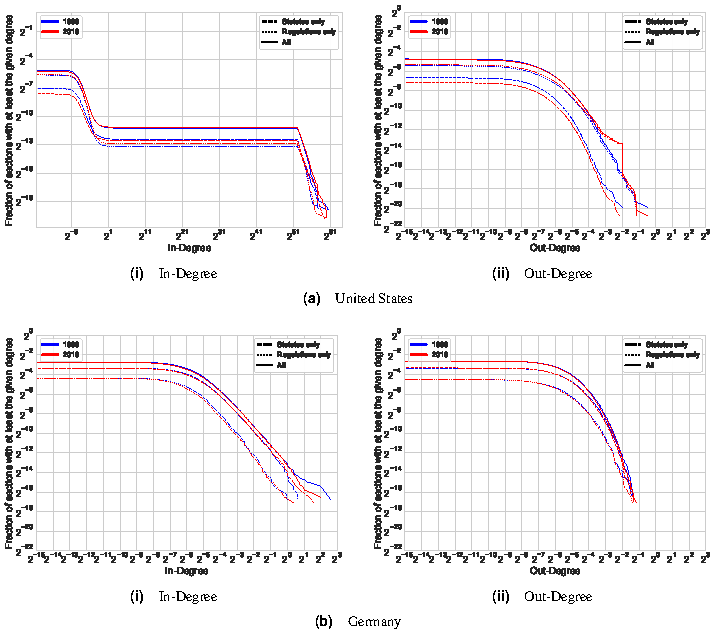
\includegraphics[width=\textwidth]{figure_si_normalized_growth}
	\caption{In-degree (left) and out-degree (right) distributions for the United States (top) and Germany (bottom) in $1998$ (blue) and $2019$ (red) when considering statutes only (dashed line), regulations only (dotted line) or statutes and regulations (solid line), normalized by section length (i.e., the plotted distributions are in-degree per token and out-degree per token).}\label{fig:growth-normalized}
\end{figure}

\vspace*{12pt}
\subsection{Growth}

The in-degree and out-degree distributions shown in the main paper do not normalize for section length.
Figure~\ref{fig:growth-normalized} provides a normalized perspective, displaying the in-degree and out-degree distributions after dividing by the sections' lengths in tokens.
The x-axis and the y-axis are shared across all panels except for the top left panel, which shows the normalized in-degree distributions for the United States.
These in-degree distributions are similar to the German in-degree distributions up to an in-degree of two references per token,
but they have a very long right tail due to a tiny number of sections with a very high number of tokens per reference.
Upon closer inspection, these sections turn out to be empty, i.e., they do not have any text at all but are still referenced by other sections in the USC or the CFR.
This is likely an artifact of the incremental codification processes in the United States, in which some Titles can be updated before others that depend on them.

\begin{figure}
	\centering
	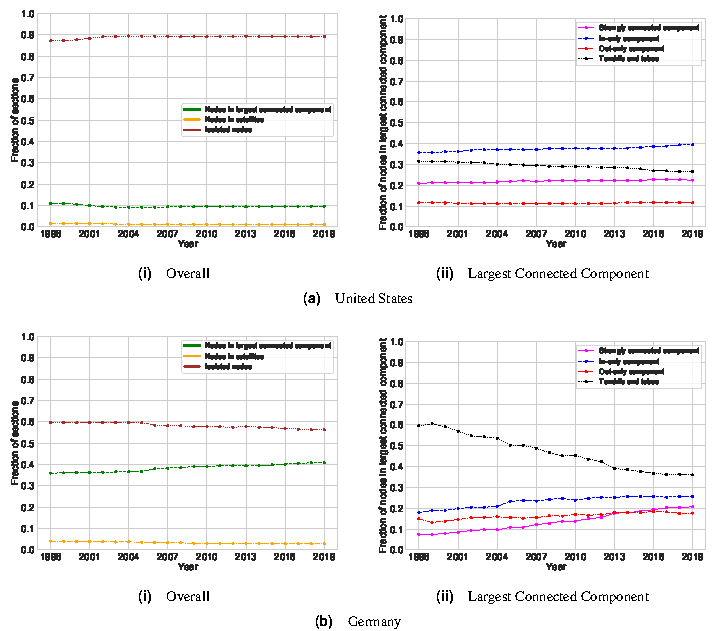
\includegraphics[width=\textwidth]{figure_si_connectivity_statutes}
	\caption{Development of reference connectivity in the United States (top) and Germany (bottom) as measured by the fraction of sections contained in the largest connected component (left) and the internal structure of that component (right) when considering \emph{statute sections only}.}\label{fig:connectivity-statutes}
\end{figure}

\vspace*{12pt}
\subsection{Macro-level connectivity}

The connectivity figures shown in the main paper depict connectivity in the graphs consisting of statutes and regulations \emph{together}.
Figure~\ref{fig:connectivity-statutes} and Figure~\ref{fig:connectivity-regulations} show connectivity for the graphs consisting of statutes only and regulations only, respectively.
The figures show that the rocket structure is nearly ubiquitous (the exception being German regulations), although the precise rocket shapes differ between the graphs.

\begin{figure}
	\centering
	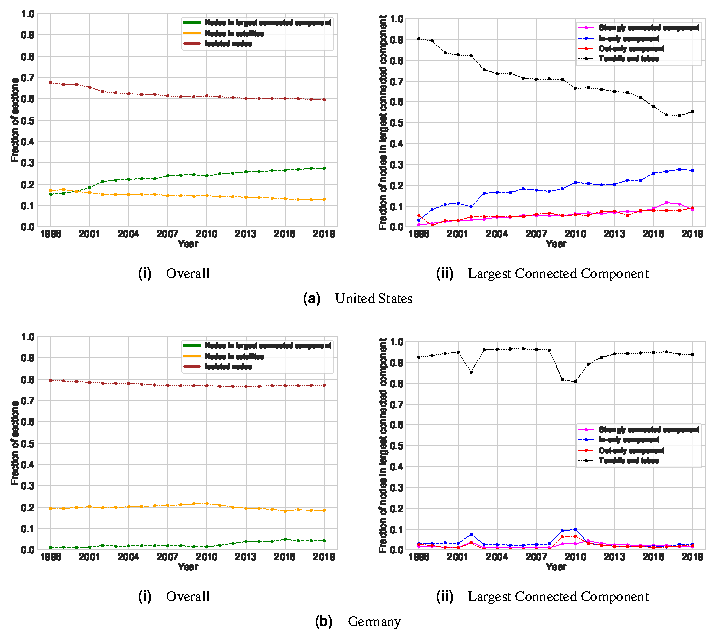
\includegraphics[width=\textwidth]{figure_si_connectivity_regulations}
	\caption{Development of reference connectivity in the United States (top) and Germany (bottom) as measured by the fraction of sections contained in the largest connected component (left) and the internal structure of that component (right) when considering \emph{regulation sections only}.}\label{fig:connectivity-regulations}
\end{figure}

%\vspace*{6pt}
\subsection{Meso-level connectivity}

\vspace*{6pt}
\subsubsection{Constructing the cluster family graph}

As input data for the clustering, we use quotient graphs on the chapter level in the United States and on the statute or regulation level (or the book level, if available) in Germany.
Especially in the CFR, there are leaf nodes containing text that do \emph{not} have a chapter as an ancestor.
We merge these nodes into the highest ancestor that does \emph{not} contain a chapter.

Computing the optimal node alignment between two graphs is generally a hard problem,
and methods based on tree edit distance do not scale to legislative trees.
However, we can use the sequence of the most granular structural elements of the statutes and regulations that we extract,
along with the text associated with individual nodes,
and exploit the fact that most rules do not change most of the time
to construct a practical heuristic that greedily computes a partial node alignment $\phi^i_t$ across two snapshots $S^i_t$ and $S^i_{t+1}$ from corpus $i$.
Building on and refining the method proposed in \cite{katz2020}, 
our heuristic operates in at most four sequential passes through these snapshots:
\begin{enumerate}
	\item \emph{First pass:}
	If $v$ is a node in $S^i_t$ and we find exactly one node $w$ in $S^i_{t+1}$ with identical text \emph{and} the text is at least 50 characters long, set $\phi^i_t(v) = w$.
	\item \emph{Second pass:}
	If $v$ is an unmatched node in $S^i_t$ and we find exactly one unmatched node $w$ in $S^i_{t+1}$ with identical key \emph{and} identical text,
	set $\phi^i_t(v) = w$.
	If no key is assigned to the node, the key of the closest ancestor will be used instead.
	\item \emph{Third pass:}
	If $v$ is an unmatched node in $S^i_t$ and we find exactly one unmatched node $w$ in $S^i_{t+1}$ such that (i) the text of $v$ contains the text of $w$ (or the text of $w$ contains the text of $v$) and (ii) the text remaining unmatched in $v$ ($w$) is shorter than the matched part, set $\phi^i_t(v) = w$.
	\item \emph{Fourth pass:}
	If $v$ is an unmatched node in $S^i_t$ and we find a matched node $v'$ in $S^i_t$ in the five-hop neighbourhood of $v$,
	search the five-hop neighborhood of $\phi^i_t(v')$ for the unmatched node $w$ (if any) with the largest Jaro-Winkler string similarity \cite{winkler1990} to $v$;
	if that similarity is above $0.9$, set $\phi^i_t(v) = w$.
	Repeat with all newly matched nodes until no further matches are found.
\end{enumerate}
To compute an alignment between individual clusters, 
we use the node alignment described above, 
leveraging that every node in this alignment belongs to a cluster. 
Therefore, we can approximate the similarity between a cluster $A$ at time $t$ and a cluster $B$ at time $t+1$ by summing up the tokens of the most granular elements that are contained in $A$ at time $t$ and aligned with $B$ at time $t+1$.

\vspace*{12pt}
\subsubsection{Cluster family labeling}
We derive the labels for the ten largest cluster families for each country from a manual inspection of their content, 
leveraging our subject matter expertise and familiarity with the United States and German legal systems.
For each country, we generate a family composition summary. 
This summary lists all clusters contained in a family, details what percentage of the cluster is made up of which particular chapter, book, statute or regulation (measured in tokens), and details the path from the root to each element contained in the family's clusters, 
including the headings of all structural elements in which it is contained.
We show the path down to the level of granularity in which we are interested, i.e., the chapter level of the USC and CFR for the United States and the book (if available), statute, or regulation level for the German data, relying on the headings to provide a description of the content.
Table~\ref{tab:family-summary} shows an excerpt from the summary of the largest cluster family in the United States as used in our manual labeling process.

\begin{table}
	\caption{Excerpt from the summary of the top cluster family, Environmental and Health Protection, as used in the manual labeling process (adapted from the HTML original).
	}\label{tab:family-summary}
	\renewcommand{\arraystretch}{1.15}
\footnotesize
\centering
\begin{tabular}{rlp{0.75\linewidth}}
    \toprule
    \multicolumn{3}{l}{\bfseries Family 0 – 2018\_10}\\
    \midrule
    \multicolumn{3}{l}{\bfseries 1998\_25}\\
    \midrule
89.14 \%&regulation	&Title 40 / Chapter I—Environmental Protection Agency\\
3.92 \%	&statute	&TITLE 42-THE PUBLIC HEALTH AND WELFARE / CHAPTER 85-AIR POLLUTION PREVENTION AND CONTROL\\
2.23 \%	&statute	&TITLE 33-NAVIGATION AND NAVIGABLE WATERS / CHAPTER 26-WATER POLLUTION PREVENTION AND CONTROL\\
1.71 \%	&regulation	&Title 40 / CHAPTER\\
1.50 \%	&statute	&TITLE 42-THE PUBLIC HEALTH AND WELFARE / CHAPTER 82-SOLID WASTE DISPOSAL\\
0.91 \%	&statute	&TITLE 7-AGRICULTURE / CHAPTER 6-INSECTICIDES AND ENVIRONMENTAL PESTICIDE CONTROL\\
0.30 \%	&statute	&TITLE 33-NAVIGATION AND NAVIGABLE WATERS / CHAPTER 27-OCEAN DUMPING\\
0.07 \%	&statute	&TITLE 42-THE PUBLIC HEALTH AND WELFARE / CHAPTER 137-MANAGEMENT OF RECHARGEABLE BATTERIES AND BATTERIES CONTAINING MERCURY\\
0.06 \%	&statute	&TITLE 16-CONSERVATION / CHAPTER 32A-REGIONAL MARINE RESEARCH PROGRAMS\\
0.05 \%	&statute	&TITLE 33-NAVIGATION AND NAVIGABLE WATERS / CHAPTER 41-NATIONAL COASTAL MONITORING\\
    \midrule
    %\\
    \dots\\
    %\\
    \midrule
    \multicolumn{3}{l}{\bfseries 2019\_14}\\
    \midrule
    80.70 \%    &regulation	&Title 40 / CHAPTER I—ENVIRONMENTAL PROTECTION AGENCY\\
    10.11 \%	&regulation	&Title 29 / Subtitle B—Regulations Relating to Labor / CHAPTER XVII—OCCUPATIONAL SAFETY AND HEALTH ADMINISTRATION, DEPARTMENT OF LABOR\\
    4.67 \%	    &regulation	&Title 49 / Subtitle B—Other Regulations Relating to Transportation / CHAPTER V—NATIONAL HIGHWAY TRAFFIC SAFETY ADMINISTRATION, DEPARTMENT OF TRANSPORTATION\\
    1.23 \%	    &statute	&TITLE 42-THE PUBLIC HEALTH AND WELFARE / CHAPTER 85-AIR POLLUTION PREVENTION AND CONTROL\\
    0.86 \%	    &statute	&TITLE 33-NAVIGATION AND NAVIGABLE WATERS / CHAPTER 26-WATER POLLUTION PREVENTION AND CONTROL\\
    0.51 \%	    &statute	&TITLE 42-THE PUBLIC HEALTH AND WELFARE / CHAPTER 82-SOLID WASTE DISPOSAL\\
    0.41 \%	    &statute	&TITLE 15-COMMERCE AND TRADE / CHAPTER 53-TOXIC SUBSTANCES CONTROL\\
    0.38 \%	    &statute	&TITLE 7-AGRICULTURE / CHAPTER 6-INSECTICIDES AND ENVIRONMENTAL PESTICIDE CONTROL\\
    0.36 \%	    &regulation	&Title 48 / CHAPTER 15—ENVIRONMENTAL PROTECTION AGENCY\\
    0.15 \%	    &statute	&TITLE 49-TRANSPORTATION / SUBTITLE VI-MOTOR VEHICLE AND DRIVER PROGRAMS / PART A-GENERAL / CHAPTER 301-MOTOR VEHICLE SAFETY\\
    \bottomrule
\end{tabular}

\end{table}

The family composition summaries provide enough dimensionality reduction to enable humans to assign a label, and they are part of the data provided with the paper. 
Supplementing this expert-based approach, 
we provide basic TF-IDF statistics (term frequency-inverse document frequency; for an introduction, see \cite{schutze2008}) for the ten largest cluster families in both countries as CSV files in the data repository accompanying this paper.
Table~\ref{tab:tfidf:part1} and Table~\ref{tab:tfidf:part2} contain the top ten nouns---according to TF-IDF (and excluding nouns describing hierarchical elements in legal texts, e.g., \emph{chapter} or \emph{section})---for the United States cluster families depicted in the main paper. 

\clearpage
 
\begin{table}
	\caption{TF-IDF statistics for the top ten cluster families with translation of abbreviations. (1 of 2)}\label{tab:tfidf:part1}
	\renewcommand{\arraystretch}{1.1}
\small
\centering
\begin{tabular}{p{0.2\linewidth}p{0.1\linewidth}p{0.1\linewidth}p{0.2\linewidth}p{0.2\linewidth}}
    \toprule
    \bfseries Environmental and Health Protection&\bfseries Healthcare and Tax&\bfseries Agriculture and Food&\bfseries Federal Grants and Commercial Activity&\bfseries Maritime Affairs and Transport\\
    \midrule
    hap             &cms       &rus         &fdic           &ocmi\\
    nox             &taxpayer  &fmha        &(o)champus     &tp\\
    cair            &income    &fns         &pbgc           &packagings\\
    emission(s)     &medicare  &aphis       &dod            &longitude\\
    voc             &qio       &premarket   &ots            &cotp\\
    pollutant       &tax       &borrower    &usaid          &commandant\\
    nonattainment   &dpgr      &swine       &occ            &liferaft\\
    cems            &annutiy   &fsa         &depository     &nls\\
    epa             &hmo       &fda         &uss            &ib\\
    kkg             &prs       &flock       &tva            &cargo\\
    \bottomrule
\end{tabular}
\vspace*{18pt}

\footnotesize
\begin{tabular}{ll}
    \toprule
    \multicolumn{2}{c}{\bfseries Environmental and Health Protection}\\
    \midrule
    hap             &Hazardous Air Pollutants\\
    nox             &Nitrogen Oxides\\
    cair            &Clean Air Interstate Rule\\
    voc             &Volatile Organic Compounds\\
    cems            &Continuous Emissions Monitoring System\\
    epa             &Environmental Protection Agency\\
    kkg             &1000 Kilograms\\   
    \midrule
    \multicolumn{2}{c}{\bfseries Healthcare and Tax}\\
    \midrule
    cms             &Centers for Medicare \& Medicaid Services\\
    qio             &Quality Improvement Organization\\
    dpgr            &Domestic Production Gross Receipts\\
    hmo             &Health Maintenance Organization\\
    prs             &Private Retirement Scheme\\
    \midrule
    \multicolumn{2}{c}{\bfseries Agriculture and Food}\\
    \midrule
    rus             &Rural Utilities Service\\
    fmha            &Farmers Home Administration\\
    fns             &Food and Nutrition Service\\
    aphis           &Animal and Plant Health Inspection Service\\
    fsa             &Farm Service Agency\\
    fda             &Food and Drug Administration\\
    \midrule
    \multicolumn{2}{c}{\bfseries Federal Grants and Commercial Activity}\\
    \midrule
    fdic            &Federal Deposit Insurance Corporation\\
    (o)champus      &(Office of) Civilian Health and Medical Programs of the Uniformed Services\\
    pbgc            &Pension Benefit Guaranty Corporation\\
    dod             &Department of Defense\\
    ots             &Officials Tracking System\\
    usaid           &United States Agency for International Development\\
    occ             &Office of the Comptroller of the Currency\\
    uss             &United States Ship\\
    tva             &Tennessee Valley Authority\\
    \midrule
    \multicolumn{2}{c}{\bfseries Maritime Affairs and Transport}\\
    \midrule
    ocmi            &Officer in Charge, Marine Inspection\\
    tp              &Time in Port\\
    cotp            &Captain of the Port\\
    nls             &Noxious Liquid Substances\\
    ib              &Invoice Book\\
    \bottomrule
\end{tabular}
\end{table}

\begin{table}
	\caption{TF-IDF statistics for the top ten cluster families with translation of abbreviations. (2 of 2)}\label{tab:tfidf:part2}
	\renewcommand{\arraystretch}{1.1}
\small
\centering

\begin{tabular}{p{0.125\linewidth}p{0.2\linewidth}p{0.15\linewidth}p{0.175\linewidth}p{0.175\linewidth}}
    \toprule
    \bfseries Financial Regulation&\bfseries Public Procurement and Funding&\bfseries Energy&\bfseries Telecommunications&\bfseries Housing\\
    \midrule
    swap(s)         &sba        &nrc                &(m$|$k$|$g)hz  &pha\\
    futures         &nasa       &doe                &antenna        &hud\\
    issuer          &hubzone    &reactor            &fcc            &mortgag(or$|$ee$|$e)\\
    registrant      &wosb       &ofe                &lec            &cdbg\\
    broker          &hsar       &uranium            &(d)tv          &homeownership\\
    dealer          &contractor &licensee           &e(i)rp         &hfa\\
    securities      &nmvc       &decommissioning    &bandwidth      &phas\\
    counterparty    &usaid      &isfsi              &transmitter    &gse\\
    sipc            &offeror    &ffd                &subscriber     &homebuyer\\
    trading         &pgi        &hrp                &px             &pae\\
    \bottomrule
\end{tabular}
\vspace*{18pt}

\footnotesize
\begin{tabular}{ll}
    \toprule
    \multicolumn{2}{c}{\bfseries Financial Regulation}\\
    \midrule
    sipc            &Securities Investor Protection Corporation\\
    \midrule
    \multicolumn{2}{c}{\bfseries Public Procurement and Funding}\\
    \midrule
    sba             &Small Business Act\\
    nasa            &National Aeronautics and Space Administration\\
    wosb            &Women-Owned Small Business\\
    hsar            &Homeland Security Acquisition Regulation\\
    nmvc            &New Model Venture Capital\\
    usaid           &United States Agency for International Development\\
    pgi             &Procedures, Guidance, and Information\\
    \midrule
    \multicolumn{2}{c}{\bfseries Energy}\\
    \midrule
    nrc             &Nuclear Regulatory Commission\\
    doe             &Department of Energy\\
    ofe             &Office of Fossil Energy\\
    isfsi           &Independent Spent Fuel Storage Installation\\
    ffd             &Fitness for Duty\\
    hrp             &Hazardous Air Pollutant\\
    \midrule
    \multicolumn{2}{c}{\bfseries Telecommunications}\\
    \midrule
    (m$|$k$|$g)hz   &(Mega$|$Kilo$|$Giga)Hertz\\
    fcc             &Federal Communications Commission\\
    lec             &Local Exchange Carrier\\
    (d)tv           &(Digital) Television\\
    e(i)rp          &Effective Isotropic Radiated Power\\
    px              &Peak Power\\
    \midrule
    \multicolumn{2}{c}{\bfseries Housing}\\
    \midrule
    pha             &Public Housing Agency\\
    hud             &U.S. Department of Housing and Urban Development\\
    cdbg            &Community Development Block Grant\\
    hfa             &Housing Finance Agency\\
    phas            &Public Housing Assessment System\\
    gse             &Government-Sponsored Enterprise\\
    pae             &Participating Administrative Entity\\
    \bottomrule
\end{tabular}
\end{table}

\clearpage

\vspace*{6pt}
\subsubsection{Cluster family categorization}

We show the exact numbers behind the classification of the top ten cluster families by their average composition or their growth,
using either the $4:1$ threshold or a simple majority rule, 
in Table~\ref{fig:family-composition} and Table~\ref{fig:family-growth}. 
As can be seen from Figure~\ref{fig:families-top-100}, 
the trends found in the inspection of the top ten families hold for the top hundred families as well. 
In the United States, the vast majority of cluster families contain less than $40~\%$ statute tokens, with a mode below $1/8$. 
Note that a substantial number of families contains statutes only, 
but while these small families make up the majority of families by number, they only account for a small fraction of the overall tokens.
In Germany, most families are also small and contain more statute tokens than regulation tokens.
Here, the larger the family, the higher the chance that it is dominated by statute tokens,
with the majority of the largest clusters containing more than $50~\%$ statutes and a mode above $7/8$. 

\begin{table}
	\caption{Family classification by average composition}\label{fig:family-composition}
	\renewcommand{\arraystretch}{1.075}
	\small\centering
	\begin{tabular}{lrrrrrrrll}
\toprule
 Family                                 &   $\mu$ &   $\sigma$ &   $\min$ &   $25~\%$ &   $50~\%$ &   $75~\%$ &   $\max$ & Cat.   & Maj.   \\
\midrule
 Environmental and Health Protection    &    0.05 &       0.02 &     0.03 &      0.04 &      0.05 &      0.06 &     0.1  & R      & R      \\
 Healthcare and Tax                     &    0    &       0    &     0    &      0    &      0    &      0    &     0.01 & R      & R      \\
 Agriculture and Food                   &    0.31 &       0.03 &     0.27 &      0.29 &      0.29 &      0.31 &     0.39 & M      & R      \\
 Federal Grants and Commercial Activity &    0.12 &       0.02 &     0.08 &      0.11 &      0.12 &      0.13 &     0.15 & R      & R      \\
 Maritime Affairs and Transport         &    0.06 &       0.01 &     0.05 &      0.06 &      0.06 &      0.07 &     0.09 & R      & R      \\
 Financial Regulation                   &    0.22 &       0.06 &     0.14 &      0.19 &      0.2  &      0.22 &     0.4  & M      & R      \\
 Public Procurement and Funding         &    0.14 &       0.02 &     0.1  &      0.13 &      0.14 &      0.15 &     0.18 & R      & R      \\
 Energy                                 &    0.29 &       0.07 &     0.21 &      0.26 &      0.27 &      0.28 &     0.58 & M      & R      \\
 Telecommunications                     &    0.15 &       0.08 &     0.11 &      0.11 &      0.12 &      0.12 &     0.36 & R      & R      \\
 Housing                                &    0.34 &       0.13 &     0.26 &      0.28 &      0.29 &      0.34 &     0.79 & M      & R      \\
\bottomrule
\end{tabular}
	
	{\vspace*{6pt}\small \textbf{\textsf{(a)}}\quad United States}\vspace*{12pt}

	\begin{tabular}{lrrrrrrrll}
\toprule
 Family                             &   $\mu$ &   $\sigma$ &   $\min$ &   $25~\%$ &   $50~\%$ &   $75~\%$ &   $\max$ & Cat.   & Maj.   \\
\midrule
 Corporations and Banking           &    0.63 &       0.04 &     0.56 &      0.59 &      0.63 &      0.67 &     0.68 & M      & S      \\
 Vocational Training                &    0.05 &       0.01 &     0.04 &      0.04 &      0.05 &      0.05 &     0.07 & R      & R      \\
 Social Security                    &    0.78 &       0.01 &     0.74 &      0.77 &      0.78 &      0.78 &     0.8  & M      & S      \\
 Courts and Data Protection         &    0.88 &       0.03 &     0.82 &      0.86 &      0.88 &      0.9  &     0.93 & S      & S      \\
 Environmental and Workplace Safety &    0.36 &       0.07 &     0.26 &      0.31 &      0.36 &      0.42 &     0.47 & M      & R      \\
 Criminal Law and Justice           &    0.9  &       0.02 &     0.84 &      0.9  &      0.91 &      0.91 &     0.93 & S      & S      \\
 Personal and Consumption Taxes     &    0.58 &       0.05 &     0.53 &      0.55 &      0.56 &      0.59 &     0.69 & M      & S      \\
 Corporate Taxes                    &    0.9  &       0.02 &     0.86 &      0.88 &      0.89 &      0.91 &     0.94 & S      & S      \\
 Environmental Protection           &    0.29 &       0.06 &     0.2  &      0.23 &      0.3  &      0.33 &     0.39 & M      & R      \\
 Property                           &    0.89 &       0.02 &     0.84 &      0.89 &      0.9  &      0.91 &     0.93 & S      & S      \\
\bottomrule
\end{tabular}
	
	{\vspace*{6pt}\small \textbf{\textsf{(b)}}\quad Germany} 
\end{table}

\begin{table}
	\caption{Family classification by growth}\label{fig:family-growth}
	\renewcommand{\arraystretch}{1.075}
	\small\centering
	\begin{tabular}{lrrrrrll}
\toprule
 Family                                 &   $\Delta$ &   $\Delta_S$ &   $\Delta_S/\Delta$ &   $\Delta_R$ &   $\Delta_R/\Delta$ & Cat.   & Maj.   \\
\midrule
 Environmental and Health Protection    &   10805178 &       217268 &                0.02 &     10587910 &                0.98 & R      & R      \\
 Healthcare and Tax                     &    7642791 &       -15410 &               -0    &      7658201 &                1    & R      & R      \\
 Agriculture and Food                   &    3746072 &       411719 &                0.11 &      3334353 &                0.89 & R      & R      \\
 Federal Grants and Commercial Activity &    3025038 &       447388 &                0.15 &      2577650 &                0.85 & R      & R      \\
 Maritime Affairs and Transport         &    2490268 &       156868 &                0.06 &      2333400 &                0.94 & R      & R      \\
 Financial Regulation                   &    1391745 &       119549 &                0.09 &      1272196 &                0.91 & R      & R      \\
 Public Procurement and Funding         &    1010815 &       161332 &                0.16 &       849483 &                0.84 & R      & R      \\
 Energy                                 &    1709216 &       287289 &                0.17 &      1421927 &                0.83 & R      & R      \\
 Telecommunications                     &    1663230 &        59303 &                0.04 &      1603927 &                0.96 & R      & R      \\
 Housing                                &     398553 &        31541 &                0.08 &       367012 &                0.92 & R      & R      \\
\bottomrule
\end{tabular}
	
	{\vspace*{6pt}\small \textbf{\textsf{(a)}}\quad United States}\vspace*{12pt}

	\begin{tabular}{lrrrrrll}
\toprule
 Family                             &   $\Delta$ &   $\Delta_S$ &   $\Delta_S/\Delta$ &   $\Delta_R$ &   $\Delta_R/\Delta$ & Cat.   & Maj.   \\
\midrule
 Corporations and Banking           &     449339 &       289601 &                0.64 &       159738 &                0.36 & M      & S      \\
 Vocational Training                &     234346 &         3267 &                0.01 &       231079 &                0.99 & R      & R      \\
 Social Security                    &     305047 &       257164 &                0.84 &        47883 &                0.16 & S      & S      \\
 Courts and Data Protection         &     252257 &       187826 &                0.74 &        64431 &                0.26 & M      & S      \\
 Environmental and Workplace Safety &     340812 &       199907 &                0.59 &       140905 &                0.41 & M      & S      \\
 Criminal Law and Justice           &     104295 &       101712 &                0.98 &         2583 &                0.02 & S      & S      \\
 Personal and Consumption Taxes     &      32480 &        76191 &                2.35 &       -43711 &               -1.35 & S      & S      \\
 Corporate Taxes                    &      80372 &        71571 &                0.89 &         8801 &                0.11 & S      & S      \\
 Environmental Protection           &     144036 &        43994 &                0.31 &       100042 &                0.69 & M      & R      \\
 Property                           &     100231 &        90412 &                0.9  &         9819 &                0.1  & S      & S      \\
\bottomrule
\end{tabular}
	
	{\vspace*{6pt}\small \textbf{\textsf{(b)}}\quad Germany} 
	\vspace*{-6pt}
\end{table}

\begin{figure}
	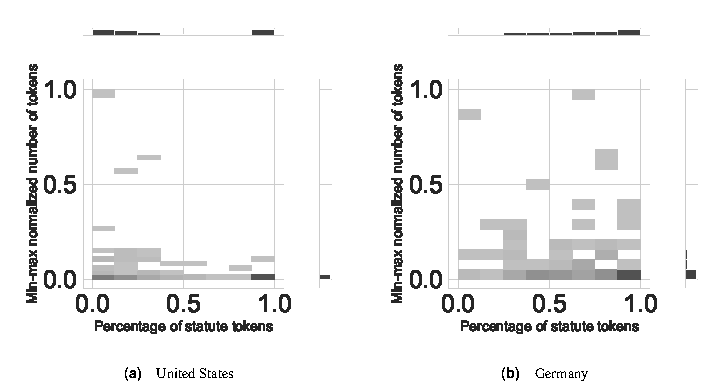
\includegraphics[width=\textwidth]{figure_si_family_top100}
	\caption{Percentage of statute tokens versus min-max normalized cluster family size in tokens for the $100$ largest families (measured in tokens) in $2019$ for the United States (left) and Germany (right).}\label{fig:families-top-100}
\end{figure}


\vspace*{12pt}
\subsubsection{Clustering algorithm parametrisation}

In the following, we analyze the performance of our clustering algorithm under different parameter choices to ensure that our results are not artifacts of our parametrization. 
The statistics we report are based on the Normalized Mutual Information (NMI) and Adjusted Rand Index (ARI)%
---two metrics that are commonly used for pairwise comparisons of clustering results.

The NMI is an information-theoretic measure expressing how much information is shared between two clusterings.
It is scaled to range between $0$ (not similar at all) and 1 (identical), and defined as
\begin{align*}
	\text{NMI}(X;Y) = \frac{I(X;Y)}{\sqrt{H(X)H(Y)}}~,
\end{align*}
where $I(X;Y) = H(X;Y)-H(X\mid Y)-H(Y\mid X)$ is the mutual information between $X$ and $Y$, $H(X;Y)$ is the joint entropy of $X$ and $Y$, 
$H(X)$ and $H(Y)$ are the individual entropies, 
and $H(X\mid Y)$ and $H(Y\mid X)$ are the conditional entropies.
For more information on this measure, see \cite{strehl2002}.

The ARI is variant of the Rand Index (RI) adjusted for chance. 
The Rand Index is based on counting how many pairs of nodes are in the same clusters or in different clusters in both clusterings. 
It is defined as
\begin{align*}
	\text{RI}(X;Y) = \frac{a+b}{a+b+c+d}~,
\end{align*}
where $a$ is the number of node pairs that appear in the same cluster in both clusterings, 
$b$ is the number of node pairs that appear in different clusters in both clusterings, 
$c$ is the number of node pairs that appear in the same cluster in $X$ but in different clusters in $Y$, and
$d$ is the number of node pairs that appear in different clusters in $X$ but in the same cluster in $Y$. 
The ARI is defined as
\begin{align*}
	\text{ARI}(X;Y) = \frac{\text{RI}(X;Y) - \mathbb{E}[\text{RI}(X;Y)]}{1 - \mathbb{E}[\text{RI}(X;Y)]}~,
\end{align*}
where $\mathbb{E}[\text{RI}(X;Y)]$ is the expected RI when assuming that the $X$ and $Y$ partitions are constructed randomly, 
subject to having the original number of clusters and the original number of nodes in each cluster.
While the RI ranges between $0$ and $1$, the ARI is bounded from above by $1$ but may take negative values when the agreement between the clusterings is less than expected. 
Unrelated clusterings have an ARI close to $0$ and identical clusterings have an ARI of $1$. 
More information on this measure can be found in \cite{hubert1985}.

\vspace*{12pt}
\paragraph{Sensitivity analysis}

Figure~\ref{fig:sensitivity-preferred-clusters} shows how the clustering results change when we alter the preferred number of clusters, 
with our chosen number of clusters as the baseline. 
As preferred numbers of clusters, we test all numbers divisible by $10$ from $10$ to $150$ as well as the number $200$. 
In one experiment, labeled \emph{auto}, we let the \emph{Infomap} algorithm choose the preferred number of clusters.
Unsurprisingly, the box plots show that clusterings become more similar to our baseline clustering with $100$ preferred clusters as we approach this number. 
At the same time, clusterings with $50$ or $200$ preferred clusters are already relatively similar to the baseline, with NMI values over $0.9$ and ARI values over $0.7$.

Note that the spread in clustering similarities is large for comparisons of the baseline with \emph{auto}, i.e., the clusterings in which \emph{Infomap} chooses the preferred number of clusters.
This is likely due to the jumps in clustering granularity that sometimes occur in \emph{Infomap} due to small differences in the minimum description length of competing models with different resolutions. 
These jumps also likely cause the spread for clusterings of the German data with a preferred number of clusters of around $20$ to $30$.
Avoiding these jumps is our primary motivation for specifying a preferred number of clusters.

%\clearpage

\begin{figure}
	\center
	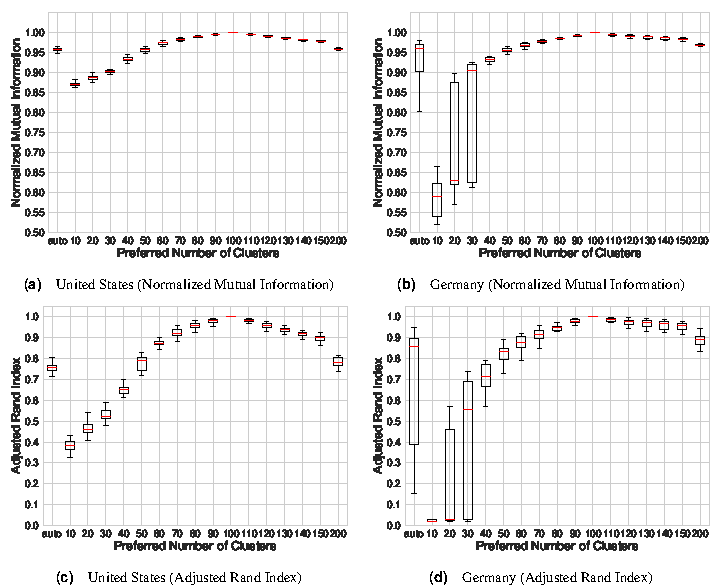
\includegraphics[width=0.9\textwidth]{figure_si_preferred_number_of_clusters.pdf}
	\caption{Distribution of pairwise similarities between clusterings with different preferred cluster sizes in the same year over the $22$ years from $1998$ to $2019$. 
		\emph{Auto} indicates that the \emph{Infomap} algorithm chooses the preferred number of clusters.
		Note that only the box plots labeled $10$ through $150$ are equidistant to each other on the real line. 
		The $y$-coordinates of the box boundaries indicate the second and fourth quartile, while the red line indicates the median. 
		Upper whiskers extend to the last data point less than $1.5$ times the box height above the fourth quartile, 
		while lower whiskers extend to the first data point less than $1.5$ times the box height below the first quartile.
	}\label{fig:sensitivity-preferred-clusters}
\end{figure}

\begin{figure}
	\center
	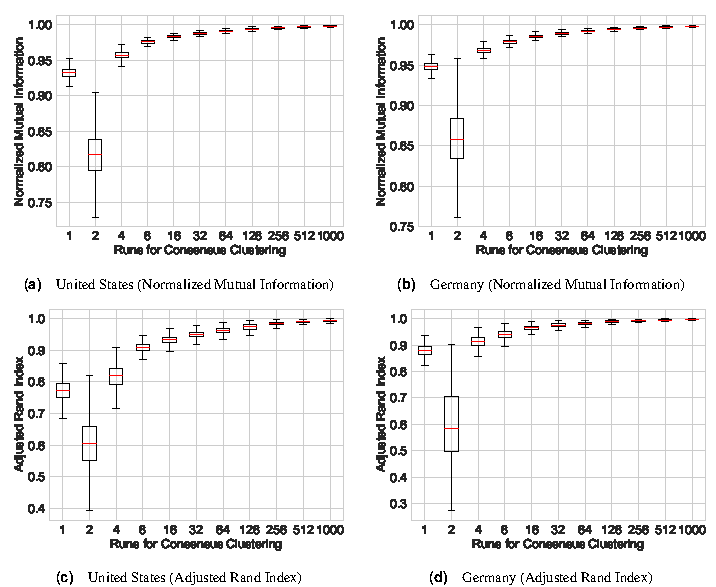
\includegraphics[width=0.9\textwidth]{figure_si_variance_impact_of_consensus_clustering.pdf}
	\caption{Pairwise similarity between $100$ consensus clustering results by number of clusterings used for finding the consensus (box plot interpretation as described in the caption of Figure~\ref{fig:sensitivity-preferred-clusters}).}
	\label{fig:consensus-effect}
\end{figure}

\vspace*{6pt}
\paragraph{Robustness checks}

Figure~\ref{fig:consensus-effect} shows the distribution of pairwise similarities between $100$ consensus clustering results for different numbers of clusterings used in the consensus. 
The plots show that using a higher number of clusterings to form the consensus increases the overall similarity level and reduces the spread between the observed similarities. 
When choosing $1000$ clusterings to form the consensus (as we do in the main paper), 
the consensus clusterings we obtain in different runs are almost identical.

Figure~\ref{fig:consensus-within} shows the distribution of pairwise similarities between $100$ pairs of clusterings (i.e., a total of $4950$ similarities) with $100$ as the preferred number of clusters. 
The NMI values for the United States clusterings mostly range between $0.85$ and $0.95$, while the NMI values for Germany mostly range between $0.88$ and $0.95$. 
The ARI values for the United States clusterings mostly range between $0.55$ and $0.85$ (with the majority lying between $0.60$ and $0.90$), 
while the ARI values for Germany mostly range between $0.75$ and $0.95$.
All similarity distributions seem to shift toward the left over time, 
i.e., clusterings in earlier years tend to be more similar to each other than clusterings in later years. 
This is likely due to the growth in complexity reported in the main paper.

\begin{figure}
	\center
	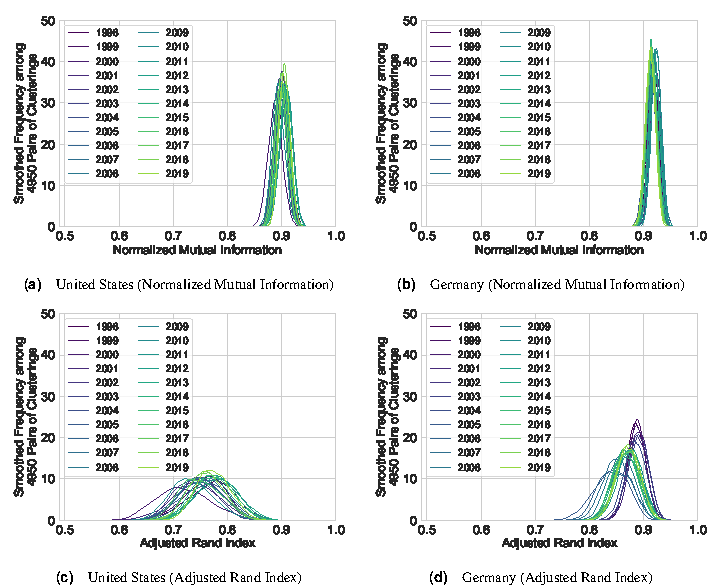
\includegraphics[width=0.9\textwidth]{figure_si_variance_infomap.pdf}
			\caption{Pairwise similarity between $100$ clusterings with $100$ as the preferred number of clusters, depicted as kernel-density estimates rather than frequency histograms to reduce visual clutter.}
	\label{fig:consensus-within}
\end{figure}

\vspace*{12pt}
\subsubsection{Cluster family evolution}

In the main paper, we show how the composition of the top ten cluster families in the United States and Germany changes over time. 
Complementing this picture, Figure~\ref{fig:sankey-us-labels} and Figure~\ref{fig:sankey-de-labels} show the evolution of the top hundred cluster families in both countries.
The figures are generated using a procedure developed in \cite{katz2020}, where it is applied to data containing only statutes.

\begin{figure}
	\centering
	\vspace*{-12pt}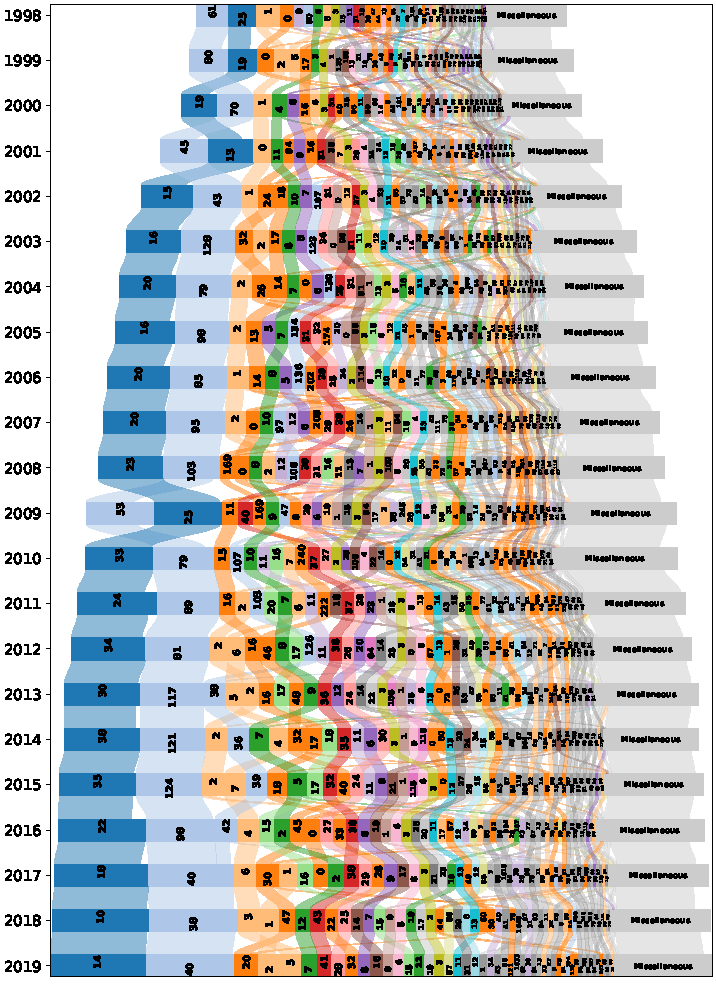
\includegraphics[width=0.9\textwidth]{figure_si_sankey_us.pdf}
	\caption{%
		Federal statutes and regulations in the United States by cluster (1998--2019), 
		with cluster numbers to enable content inspection. 
		Each block in each year represents a cluster. 
		Clusters are ordered from left to right by decreasing size (measured in tokens) and colored by the cluster family to which they belong, 
		where clusters not in one of the $20$ largest cluster families are colored in alternating greys. 
		Small clusters are summarized in one miscellaneous cluster, which is always the rightmost cluster and colored in light grey.
	}
	\label{fig:sankey-us-labels}
\end{figure}

\begin{figure}
	\centering
	\vspace*{-12pt}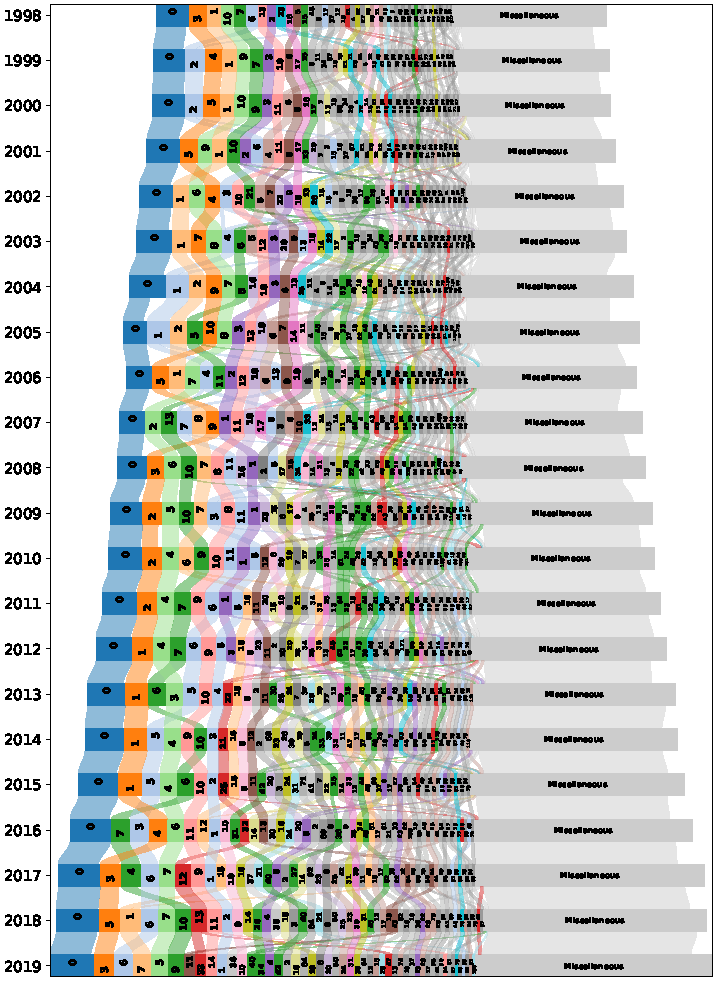
\includegraphics[width=0.9\textwidth]{figure_si_sankey_de.pdf}
	\caption{%
		Federal statutes and regulations in Germany by cluster (1998--2019), 
		with cluster numbers to enable content inspection. 
		Each block in each year represents a cluster. 
		Clusters are ordered from left to right by decreasing size (measured in tokens) and colored by the cluster family to which they belong, 
		where clusters not in one of the $20$ largest cluster families are colored in alternating greys. 
		Small clusters are summarized in one miscellaneous cluster, which is always the rightmost cluster and colored in light grey.
	}
	\label{fig:sankey-de-labels}
\end{figure}



\vspace*{12pt}
\subsection{Profiles}
In the main paper, we show the profiles of selected statutes and regulations in a case study on financial regulation. 
Complementing this analysis, Figure~\ref{fig:si-profile-trends} depicts the macro-level trends we observe in the United States data as indicated by the individual and pairwise joint distributions of the changes (value in $2019$ minus value in $1998$) in seven of our ten indicators, for all USC and CFR chapters that exist in both $1998$ and $2019$.
By excluding chapters added after $1998$, we ensure that we measure growth over the same interval for all chapters.
Figure~\ref{fig:si-profile-trends} reveals, inter alia, that the change distributions are generally more concentrated for statutes than they are for regulations, and that the joint change distribution of \emph{binary in-degree} and \emph{items on section level} best (visually) separates statutes and regulations.
Furthermore, outliers in the (growth of) size and self-referentiality are mostly regulations, while outliers in in-degree indicators are mostly statutes, and outliers in out-degree indicators are of mixed document types.
For illustration, Table~\ref{tab:si-profile-trends} lists the USC or CFR chapters that experienced the largest absolute increase from $1998$ to $2019$ in one of our ten indicators.


\begin{figure}
	\centering
	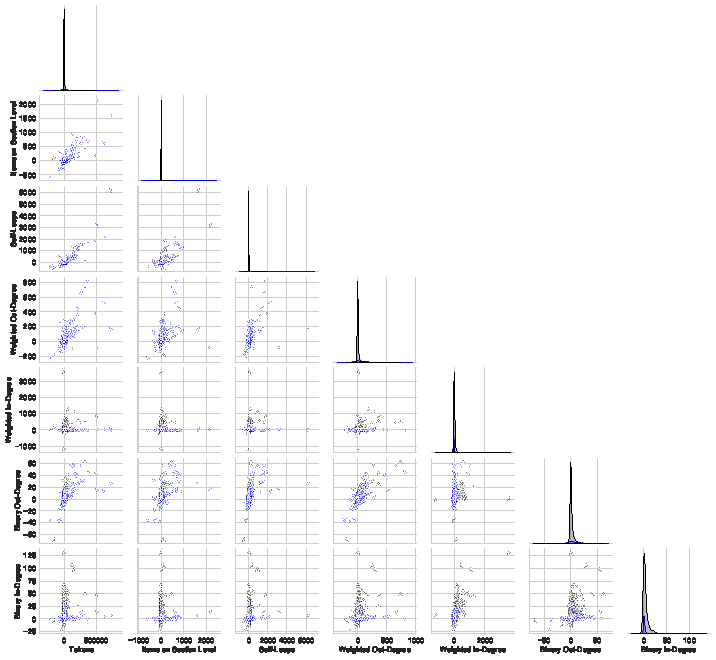
\includegraphics[width=\textwidth]{figure_si_profile_trends.pdf}
	\caption{%
	Individual distribution (diagonal) and pairwise joint distribution (lower triangle) of changes in profile variables for USC (black) and CFR (blue) chapters present in $1998$ and $2019$, for seven of the ten indicators introduced in the main paper.
	}\label{fig:si-profile-trends}
\end{figure}

\begin{table}
	\centering
	\small
	\caption{%
	Chapters of the USC and the CFR that experienced the largest absolute increase from $1998$ to $2019$ in one of the ten indicators introduced in the main paper, with CFR chapters marked grey.}\label{tab:si-profile-trends}
	\begin{tabular}{lp{0.625\textwidth}r}
		\toprule
		\textbf{Indicator}&\textbf{Chapter}&\textbf{$\Delta$}\\
		\midrule
		\rowcolor{lightgray!30}Tokens & 10 CFR Ch. I—NUCLEAR REGULATORY COMMISSION & 734462\\
		\rowcolor{lightgray!30}Unique tokens & 49 CFR Ch. V—NATIONAL HIGHWAY TRAFFIC SAFETY ADMINISTRATION, DEPARTMENT OF TRANSPORTATION & 27090\\\midrule
		\rowcolor{lightgray!30}Items above Section Level & 14 CFR Ch. I—FEDERAL AVIATION ADMINISTRATION, DEPARTMENT OF TRANSPORTATION & 301\\
		\rowcolor{lightgray!30}Items on Section Level & 14 CFR CHAPTER I—FEDERAL AVIATION ADMINISTRATION, DEPARTMENT OF TRANSPORTATION & 2152\\
		Items below Section Level & 42 USC Ch. 7—SOCIAL SECURITY & 22188\\\midrule
		\rowcolor{lightgray!30}Self-Loops & 10 CFR Ch. I—NUCLEAR REGULATORY COMMISSION & 6193\\\midrule
		\rowcolor{lightgray!30}Weighted Out-Degree & 12 CFR Ch. III—FEDERAL DEPOSIT INSURANCE CORPORATION & 817\\
		Weighted In-Degree & 5 USC Ch. 5—ADMINISTRATIVE PROCEDURE & 3580\\\midrule
		Binary Out-Degree & 42 USC Ch. 6A—PUBLIC HEALTH SERVICE & 62\\
		Binary In-Degree & 5 USC Ch. 5—ADMINISTRATIVE PROCEDURE & 131\\
		\bottomrule
	\end{tabular}
\end{table}

The profiles of individual statutes and regulations primarily serve to track their development over time.
Over the course of the analysis, however, we found that they are also helpful in highlighting potential problems with our dataset.
As visualized in Figure~\ref{fig:si-profile-17-cfr-ii},
17~CFR~Ch.~II, which deals with the Securities and Exchange Commission, displays some astonishing dynamics:
All metrics drop to varying degrees in $2002$ and $2003$, then rebound in $2004$.
Similarly, in $2016$, all these statistics fall sharply before rising back in $2017$.

Investigating these shifts, we find that they are indeed contained in the data.
In $2003$, large parts of 17~CFR~Ch.~II are contained within a tag designated \texttt{<SUPERSED>}, which---based on a comment in the document type definition---is used for ``superseded material''.
Since the relevant parts reappear in $2004$, we suspect that the closing tag is misplaced or missing.
As our extraction correctly disregards text within \texttt{<SUPERSED>} tags, all metrics drop depending on their sensitivity to lost text within this specific chapter.
The drop in $2016$ can be explained by a similar problem with a presumably accidentally extended \texttt{<REVTXT>} tag,
which---based on a comment in the document type definition---is used for ``text that is revised''.
This text, too, is not included in a \texttt{<REVTXT>} tag in the following year.
Both dynamics are therefore artifacts, which---once identified---could be mitigated by applying suitable rules or using the \emph{forward fill} strategy devised in Section~\ref{subsec:uscfr}.
We choose a separate regulation to demonstrate our framework in the main text and detail our observations here to help improve data quality over time.

A separate issue is indicated by the sharp spike in weighted in-degree, accompanied by a modest rise in binary in-degree, in $2009$.
Upon closer inspection, this increase stems from the fact that our data for this year contains a separate node titled ``17~CFR~Ch.~II~(CONTINUED)'' indicating that-–-as happens from time to time-–-the raw data contains two separate files that both contain text for the chapter in question.
We estimate the overall effect of this unexpected phenomenon, which occurs a total of fifteen times in the data,\footnote{%
The affected (sub)chapters are (in chronological, then numerical order):
43~CFR~Ch.~II ($1998$),
26~CFR~Subch.~A ($1998$),
26~CFR~Ch.~1 ($2000$-$2002$),
46~CFR~Ch.~I ($2006$, twice),
43~CFR~Ch~.~II ($2008$),
17~CFR~Ch.~II ($2009$),
42~CFR~Ch.~IV ($2009$),
10~CFR~Ch.~I ($2009$),
21~CFR~Ch.~I ($2009$), and
26~CFR~Ch.~I ($2009$, thrice).
} to be negligible for the overall analysis.
However, this needs to be addressed in future work, and it serves as a reminder that, despite the best efforts of the bodies managing the codification processes, the data quality can still be improved.
In the past, the respective public offices have been open toward and grateful for deficiencies pointed out by quantitative researchers,
and we will work with the U.S. Government Publishing Office to remove the errors we identify.

\begin{figure}
	\centering
	\vspace*{0pt}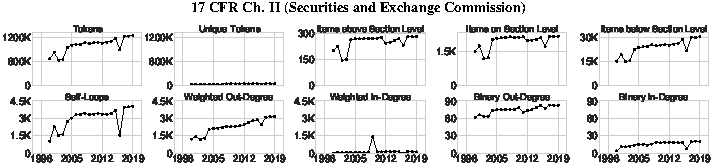
\includegraphics[width=\textwidth]{figure_si_profiles.pdf}
	\caption{%
		Profile tracking the evolution of 17 CFR Ch. II (Securities and Exchange Commission),
		including several indicators highlighting data quality problems.
	}
	\label{fig:si-profile-17-cfr-ii}
\end{figure}

\newpage

% \section{Supplementary Data}

% Supplementary Material should be uploaded separately on submission. Please include any supplementary data, figures and/or tables. All supplementary files are deposited to FigShare for permanent storage and receive a DOI.

% Supplementary material is not typeset so please ensure that all information is clearly presented, the appropriate caption is included in the file and not in the manuscript, and that the style conforms to the rest of the article. To avoid discrepancies between the published article and the supplementary material, please do not add the title, author list, affiliations or correspondence in the supplementary files.

% \section{Supplementary Tables and Figures}

% For more information on Supplementary Material and for details on the different file types accepted, please see \href{http://home.frontiersin.org/about/author-guidelines#SupplementaryMaterial}{the Supplementary Material section} of the Author Guidelines.

% Figures, tables, and images will be published under a Creative Commons CC-BY licence and permission must be obtained for use of copyrighted material from other sources (including re-published/adapted/modified/partial figures and images from the internet). It is the responsibility of the authors to acquire the licenses, to follow any citation instructions requested by third-party rights holders, and cover any supplementary charges.

% %% Figures, tables, and images will be published under a Creative Commons CC-BY licence and permission must be obtained for use of copyrighted material from other sources (including re-published/adapted/modified/partial figures and images from the internet). It is the responsibility of the authors to acquire the licenses, to follow any citation instructions requested by third-party rights holders, and cover any supplementary charges.

% \subsection{Figures}

% %%% There is no need for adding the file termination, as long as you indicate where the file is saved. In the examples below the files (logo1.eps and logos.eps) are in the Frontiers LaTeX folder
% %%% If using *.tif files convert them to .jpg or .png
% %%%  NB logo1.eps is required in the path in order to correctly compile front page header %%%

% \begin{figure}[htbp]
% \begin{center}
% %
\includegraphics[width=9cm]{logo1}% This is a *.eps file
% \end{center}
% \caption{ Enter the caption for your figure here.  Repeat as  necessary for each of your figures}\label{fig:1}
% \end{figure}


% \begin{figure}[htbp]
% \begin{center}
% %\includegraphics[width=10cm]{logos}
% \end{center}
% \caption{This is a figure with sub figures, \textbf{(A)} is one logo, \textbf{(B)} is a different logo.}\label{fig:2}
% \end{figure}

%%% If you are submitting a figure with subfigures please combine these into one image file with part labels integrated.
%%% If you don't add the figures in the LaTeX files, please upload them when submitting the article.
%%% Frontiers will add the figures at the end of the provisional pdf automatically
%%% The use of LaTeX coding to draw Diagrams/Figures/Structures should be avoided. They should be external callouts including graphics.


%\bibliographystyle{frontiersinSCNS_ENG_HUMS} %  for Science, Engineering and Humanities and Social Sciences articles, for Humanities and Social Sciences articles please include page numbers in the in-text citations
\bibliographystyle{frontiersinHLTH&FPHY} % for Health and Physics articles
\bibliography{bibliography.bib}


\end{document}
